%Centralizar verticalmente.
\newenvironment{midpage}{\vspace*{\fill}}{\vspace*{\fill}}
%Centralizar horizontalmente.
\newenvironment{midline}{\hspace*{\fill}}{\hspace*{\fill}}
\documentclass[12pts]{article}
\usepackage[utf8]{inputenc} 
\title{
	Prática de Eletrônica Digital 1 - (119466)
	\singlespacing
		Turma E (Unb - Gama)
	\singlespacing
	\begin{midpage}
	\begin {large}
		Relatório Experimento 1
		\singlespace
		Portas Lógicas
	\end {large}
	\end{midpage}
}
\date{Agosto 20, 2016}
\usepackage{indentfirst}
\usepackage{setspace}
\usepackage{verbatim}
\usepackage[pdftex]{hyperref}
\usepackage{graphicx}
\begin{document}
\maketitle	
%\vspace{100 mm}
\begin{center}

\begin{tabular}{|c|l|r|}
\hline
Nome & Matrícula & Assinatura\\
\hline
Arthur Temporim & 140016759 & \\
\hline	
Eduardo Nunes & 140056189 & \\
\hline	
\end{tabular}

\end{center}


\newpage

\section{Sumário}

\begin{itemize}
	\item Introdução
	\singlespacing
	\item Parte Experimental
	\singlespacing
	\item Discussão
	\singlespacing
	\item Conclusões 
	\singlespacing
	\item Referências Bibliograficas
	\singlespacing
	%\item Diagramas esquemáticos
\end{itemize}

\newpage


\section{Introdução}
\iffalse
Introdução, indicando a delimitação do tema, apresentando a justificativa descrevendo o propósito do relatório.
\fi
	Neste relatório é apresentado os passos seguidos para conseguir elaborar o primeiro experimento da disciplina de prática da eletrônica digital 1.

	São apresentados passos de configuração do ambiente com o \textit{Ise design suite}, imagens com as pequenos projetos simulados e comparações entre métodos de implementação de circuitos com o \textit{Ise Design Suit} e com o \textit{Qucs}.

\section{Procedimentos}
\iffalse
Parte Experimental, descrevendo os passos realizados, dificuldades e soluções para os problemas encontrados. Aqui, deve-se apresentar uma descrição dos resultados encontrados em forma de figuras, gráficos e tabelas.
\fi

\textbf{1. Os passos seguidos para configurar o ambiente de simulação}

\singlespacing

\textbf{Passo 01:} A primeira ação a se fazer para se iniciar um projeto é criar o projeto. Portanto, no menu "File", clica-se em "New Project...". 
Consequência: É aberta a janela para se criar um novo projeto no qual iremos colocar partir para o passo 2
\singlespacing

\textbf{Passo 02:} Deve se prencher o nome do projeto que será criado e colocar a localização dentre os diretórios o qual ele deve ser criado. Deve se também selecionar na combobox inferior o tipo de arquivo que será trabalhado no caso foi selecionado "Schematic". Clicamos no botão inferior: "Next".
Consequência: Somos direcionados a uma outra janela, no caso, esta referece as configurações do projeto. Vamos preservar as configurações default.
\singlespacing

\textbf{Passo 03:} Clicamos em "Next". Não alterando nenhuma configuração do projeto. 
Consequência: É exibido um sumário a respeito das configurações do ambiente que foram feitas. Basta conferir se, realmente, neste expõe a configuração que foram feitas ao projeto. Se sim, basta finalizar a criação do projeto apertando no botão inferior: "Finish". Caso contrário, as configurações exibidas não refletem a sua vontade de configuração basta voltar, clicando no botão inferior: "Back", e configurar seguindos estes passos novamente. 
\singlespacing

\textbf{Passo 04:} Com os passos anteriores finalizados, basta criar um novo projeto para iniciar as simulações.
\singlespacing

\newpage
\textbf{2. As telas capturadas durante as atividades no ambiente de laboratório;}
\singlespacing

\textbf{Atividade 01: NAND}

\begin{figure}[!htb]
  \centering
  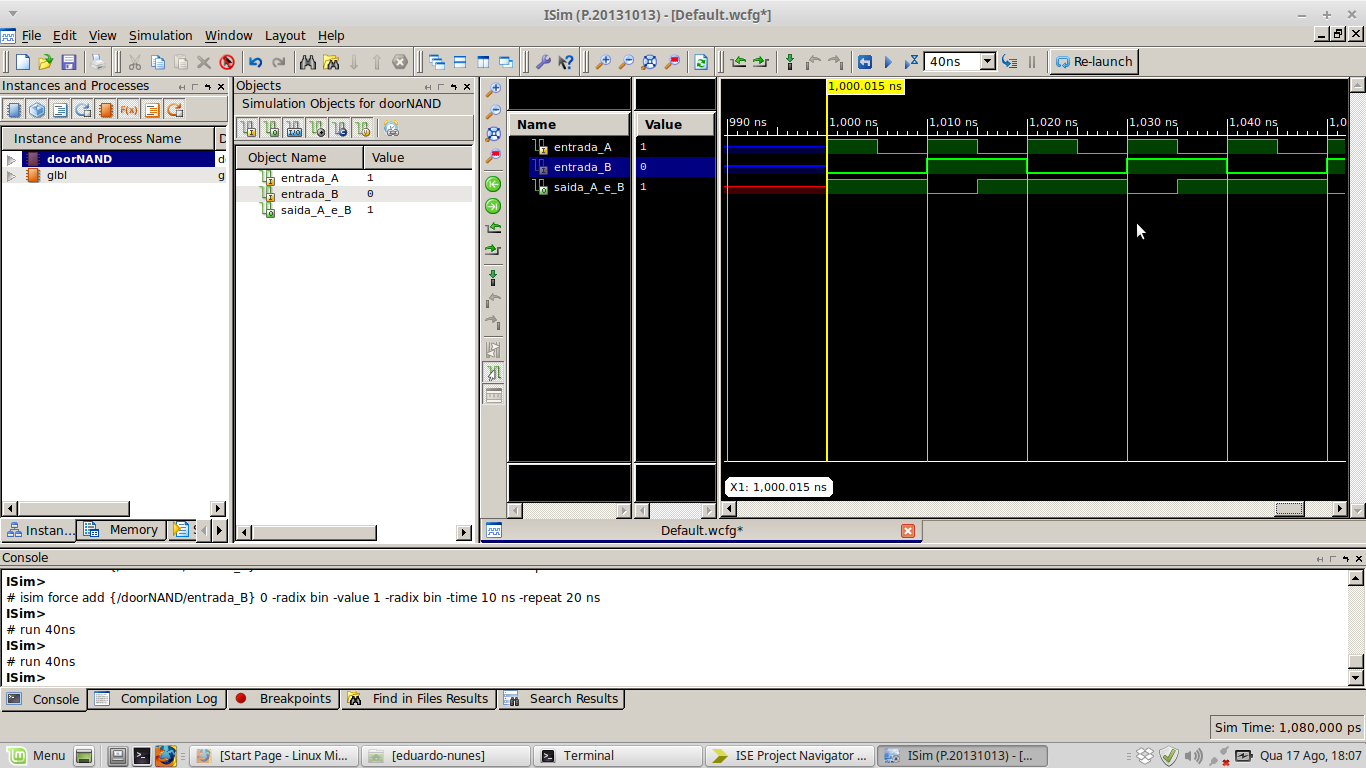
\includegraphics[scale=0.3]{Atividade01}
  \caption{Diagrama de ondas NAND - Ise Design Suite 14.7}
  \label{figRotulo}
\end{figure}

\newpage
\textbf{Atividade 02: XNOR}

\begin{figure}[!htb]
  \centering
  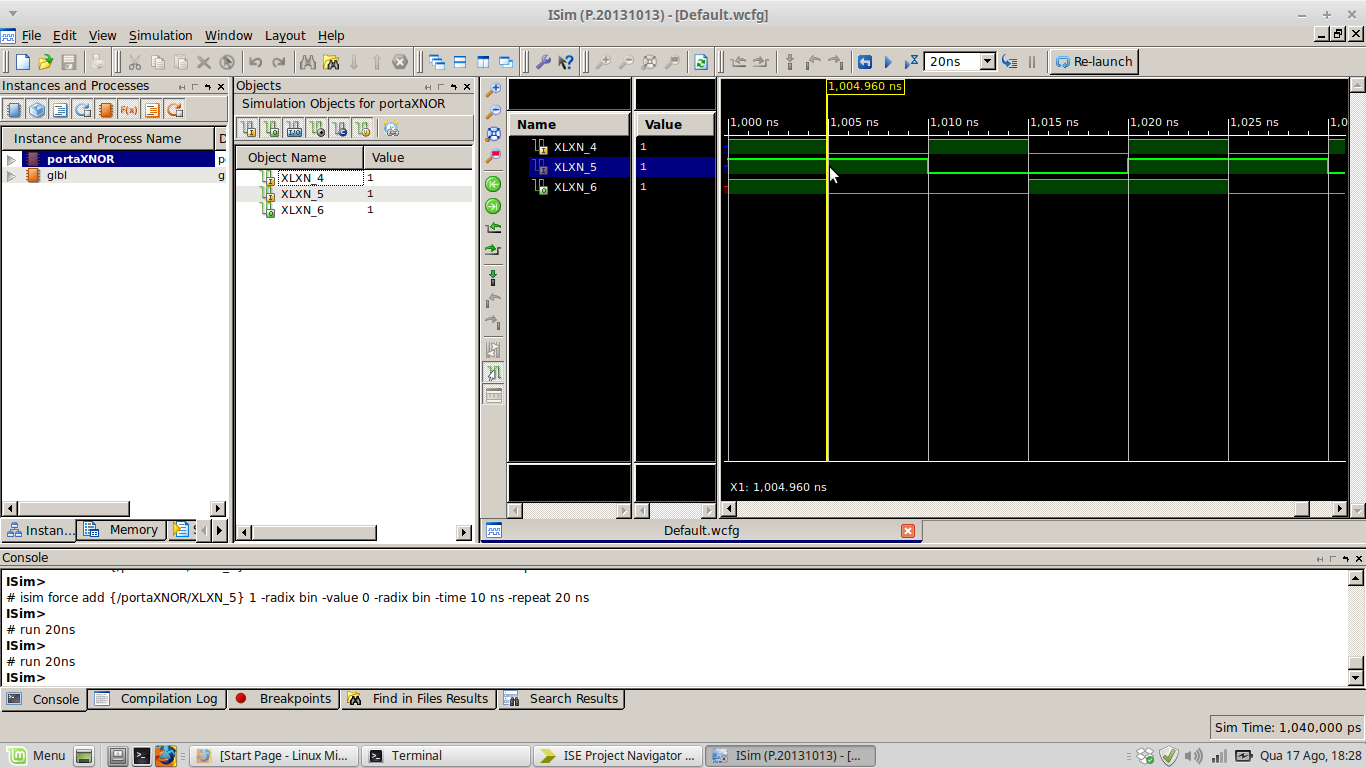
\includegraphics[scale=0.3]{Atividade02}
  \caption{Diagrama de ondas XNOR - Ise Design Suite 14.7}
  \label{figRotulo}
\end{figure}
\singlespacing

Tabela Verdade XNOR:

\begin{center}
	\begin{tabular}{|r|r|r|}
		\hline
		A & B & S\\
		\hline
		0 & 0 & 1\\
		\hline
		0 & 1 & 0\\
		\hline
		1 & 0 & 0\\
		\hline
		1 & 1 & 1\\
		\hline
	\end{tabular}
\end{center}

\newpage
\textbf{Atividade 03: NAND e XNOR em VHDL}
\singlespacing

	Na imagem abaixo contém o diagrama de ondas das duas portas feitas em VHDL. É possível notar que o resultado final é o mesmo que os anteriores.

\begin{figure}[!htb]
  \centering
  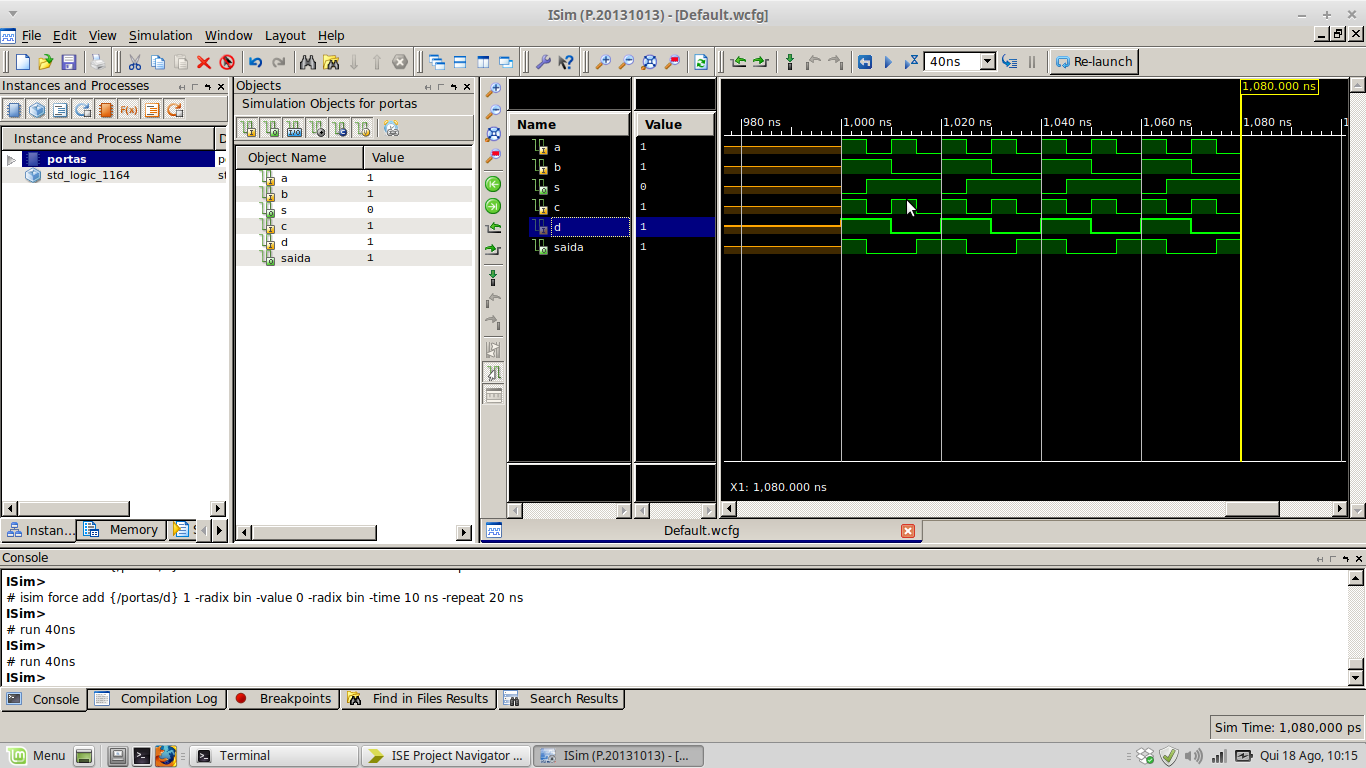
\includegraphics[scale=0.3]{Atividade03}
  \caption{Diagrama de ondas NAND e XNOR - Ise Design Suite 14.7}
  \label{figRotulo}
\end{figure}

\newpage
\textbf{Atividade 04: AND3}

\begin{figure}[!htb]
  \centering
  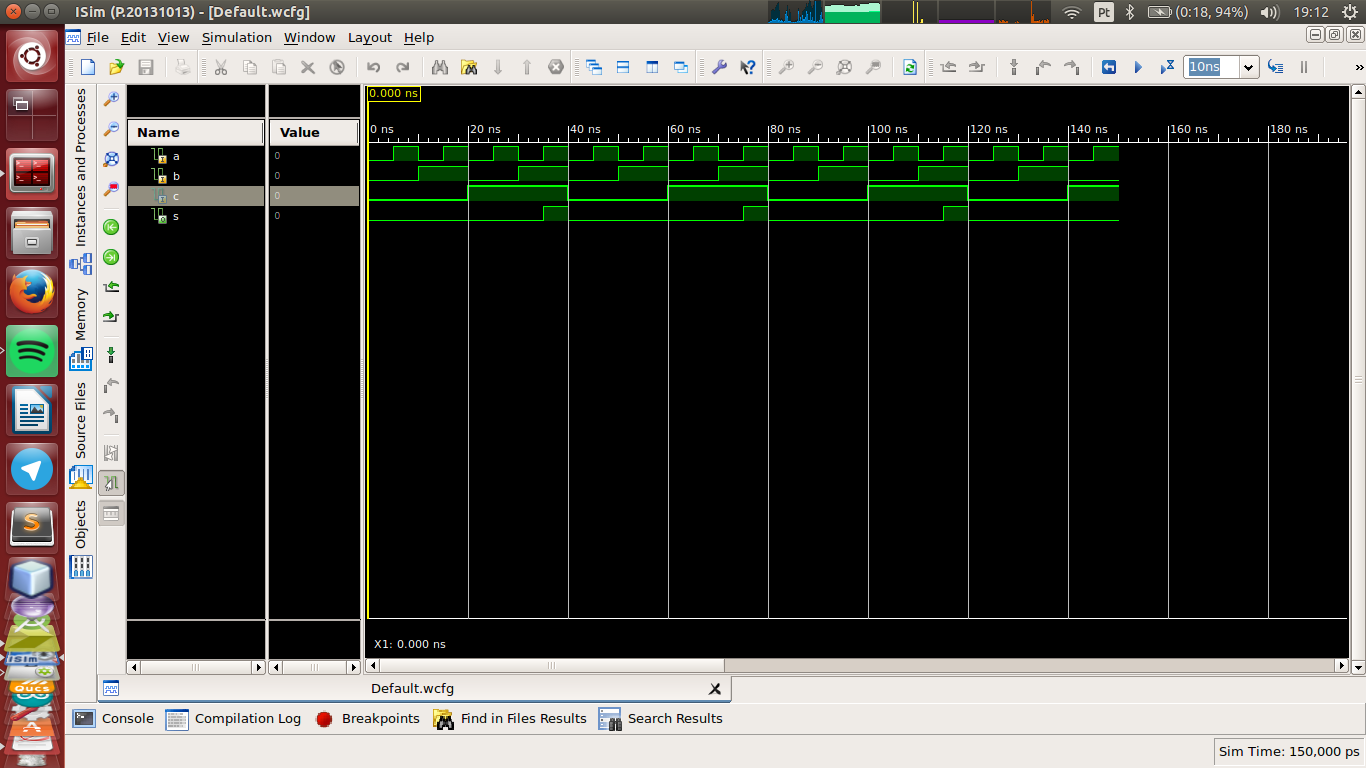
\includegraphics[scale=0.3]{Atividade04}
  \caption{Diagrama de ondas AND3 - Ise Design Suite 14.7}
  \label{figRotulo}
\end{figure}

Tabela Verdade AND3:

\begin{center}
	\begin{tabular}{|r|r|r|r|}
		\hline
		A & B & C & S\\
		\hline
		0 & 0 & 0 & 0\\
		\hline
		0 & 0 & 1 & 0\\
		\hline
		0 & 1 & 0 & 0\\
		\hline
		0 & 1 & 1 & 0\\
		\hline
		1 & 0 & 0 & 0\\
		\hline
		1 & 0 & 1 & 0\\
		\hline
		1 & 1 & 0 & 0\\
		\hline
		1 & 1 & 1 & 1\\
		\hline
	\end{tabular}
\end{center}

\newpage
\textbf{3. Uma comparação entre os métodos de descrição das portas lógicas (circuito usando símbolos lógicos, tabela-verdade, expressão booleana, código VHDL);}
\singlespacing

	A partir da tabela-verdade é capaz de se analisar uma ou mais conjutos de portas lógicas individualmente. É um forma eficiente para listar as possíveis combinações de entrada.

	Expressão booleana possibilita desenhar com maior facilidade o diagrama do circuito, pois a visualização das portas que serão necessarias para construir um circuito é melhor evidenciado. Já o código VHDL, facilita a projeção da implementação de um circuito lógico.

\singlespacing
\textbf{4. Simulação do circuito da Atividade 4 em um simulador diferente do usado em sala, apresentando as formas de onda correspondentes. Compare os dois simuladores levando em conta os seguintes aspectos:}
\singlespacing

	Esta atividade foi feita utilizando o Software \textit{Qucs}. Segue abaixo uma imagem com o resultado da utilização do programa:
	
\begin{figure}[!htb]
  \centering
  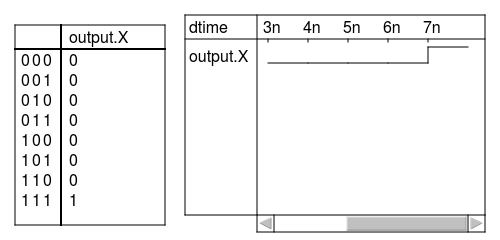
\includegraphics[scale=1]{qucs}
  \caption{Diagrama de ondas AND3 - Qucs}
  \label{figRotulo}
\end{figure}
	
	
\begin{itemize}
	\item \textbf{Facilidade de uso;}
	
	O Qucs, é bem mais leve e rápido ao ser comparado com o \textit{Ise Design Suit}, porém seu uso não é intuitivo. Com o \textit{Drag an Drop} seu uso fica mais fácil mas não é uma tarefa simples adicionar cada componente e navegar no seu menu como na outra ferramenta.
	
	\item \textbf{Possibilidade de uso de VHDL;}
	
	O \textit{Qucs} também contém a utilizaçao do VHDL para implementação de circuitos.
	
	\item \textbf{Flexibilidade na apresentação dos resultados desejados.}
\end{itemize}

	A apresentação dos resultados e a flexibilidade de vizualização é muito melhor com o \textit{Ise Design Suit}, podendo alterar o intervalo do diagrama de onda, cor e valor das entradas instantaneamente.


\section{Discussão}
\iffalse
Discussão sobre os resultados encontrados, comentando detalhadamente as medições realizadas e dando a devida interpretação destas, informando se os objetivos da experimento foram alcançados. Esta é uma das partes mais importantes do relatório: aqui, há oportunidade para expressar os conhecimentos adquiridos na prática e fazer a interrelação com os fundamentos teóricos.
\fi

	Com a realização deste experimento foi possível adquirir o primeiro contato com o ambiente de descrição de hardware com o VHDL e implementação da parte mais primitiva dos circuitos lógicos, as portas lógicas.
	
	O icentivo de 2 programas distintos para a realização da mesma atividade também foi relevante para o aprendizado da dupla e compreensão da implementação de circuitos.

\section{Conclusões}
\iffalse
Conclusões, mostrando os êxitos e eventuais problemas encontrados na realização do experimento, indicando as limitações, apresentando recomendações e/ou sugestões.
\fi

	Neste primeiro relatório foi possível realizar todas as atividade com êxito sem dificuldades significativas.

\section{Referências Bibliográficas}
\iffalse
Referencias Bibliográficas, relacionadas e citadas de acordo com as normas da ABNT.
\fi
Prática de Eletrônica Digital I 2016.2 professores Henrique Marra Taira Menegaz,Leonardo Aguayo, Lourdes Mattos Brasil, Marcus Vinícius Chaffim Costa, Mariana Costa Bernardes Matias. UnB - FGA Agosto de 2015.

\iffalse
\section{Diagramas Esquemáticos}
Diagramas Esquemáticos. Todos os diagramas devem ser inseridos ao final do relatório em páginas separadas do texto, indicando a identificação do circuito, autor, revisor, versão e datas relevantes.
\fi
\newpage
\end{document}

%Exemplo de imagem
\iffalse
\begin{figure}[!htb]
  \centering
  \includegraphics[scale=0.3	]{nome_da_imagem}
  \caption{Descrição}
  \label{figRotulo}
\end{figure}
\fi

% Exemplo de tabela.
\iffalse
\begin{tabular}{|c|r|}
\hline
Material Utilizado & Quantidade\\
\hline
Cabo Banana-Banana & 2  \\
\hline
Fios de cobre & x \\
\hline
Cabo coaxial & 3  \\
\hline
CI 74HC00   & 1 \\
\hline
CI 74LS00   & 1 \\
\hline
Protoboard & 2 \\
\hline
Fonte de tensão MPL-3305M & 1 \\
\hline	
Multímetro Digital  & 1 \\
\hline
Gerador de funçoes iCEL modelo GV-2002 & 1 \\
\hline
Osciloscopio BK 2530 & 1 \\
\hline
\end{tabular}
\singlespacing
\fi